\documentclass["../Cours.tex"]{subfiles}

\begin{document}

\begin{center}
    {\Huge Fiche de révision n°1}    
\end{center}


\thispagestyle{empty}

\color{black}

\begin{questions}
    \exercicetitre{Lecture graphique}

    L'INSEE (Institut National de Statistiques et des Études Économiques) fournit le graphique ci-dessous à l'adresse suivante :  {\tiny{https://www.insee.fr/fr/outil-interactif/5367857/details/90\_DDE/92\_DEV/92G\_Figure7}}

    \begin{center}
        \begin{tikzpicture}[yscale=0.3,xscale=2]
            \draw (-0.5,-7) rectangle (8,16);
            \node at (3.85,14.5) {\large{\bfseries Émissions de gaz à effet de serre par habitant en France}};
            \draw[-Latex] (0,0) -- (7.7,0);
            \foreach[count=\i] \annee/\valeur/\valeurf in {1995/11.2/8.9, 2000/11.0/8.8, 2005/11.0/8.5, 2010/10.4/7.5, 2015/9.3/6.6, 2020/8.3/5.6, 2021/8.9/6.0} {
                \node[below] at (\i,0) {\annee};
                \fill[noir] ({\i-0.4},0) rectangle ({\i},\valeur);
                \fill[gray] ({\i+0.4},0) rectangle ({\i},\valeurf);
            }
            \draw[-Latex] (0,0) -- (0,13);
            \foreach \y in {2,4,6,8,10,12} {
                \draw (-0.1,\y) node[left]{\y} -- +(0.2,0);
                \draw[dotted] (0.1,\y) -- (7.7,\y);
                \draw[dotted] (0,\y-1) -- (7.7,\y-1);
            }
            \fill[noir] (0,-3) rectangle +(0.5,-1) node[yshift=1ex,right]{Empreinte carbone (en tonnes équivalent $CO_2$ par habitant)};
            \fill[gray] (0,-5) rectangle +(0.5,-1) node[yshift=1ex,noir,right]{Émission sur le territoire national (en tonnes équivalent $CO_2$ par habitant)};
        \end{tikzpicture}
    \end{center}

    \textit{Exemple de lecture :} En 2021, l'empreinte carbone pour les 3 principaux gaz à effet de serre ($CO_2$, $CH_4$ et $N_2O$) s'élève à environ 9 tonnes équivalent $CO_2$ par habitant.

    \question À combien s'élève l'empreinte carbone par habitant en 2000 ?
    \question À combien s'élève l'émission sur le territoire national par habitant en 2021 ?
    \question Quelle est la différence entre << l'empreinte carbone >> et << l'émission sur le territoire national >> ?
    \question Globalement, les émissions de gaz à effet de serre ont augmenté ? diminué ? Expliquer.

    \exercicetitre{Périmètres et aires}
    Dans cet exercice, le codage << $\times$ >> correspond à une longueur de \qty{3}{\centi\metre}.

    \begin{center}
        \begin{tikzpicture}
            \draw (0,0) -- ++(3,0) node[midway]{$\times$} node[below]{\qty{3}{\centi\metre}} -- ++({3*cos(30)},{3*sin(30)}) node[midway]{$\times$} --  ++({3*cos(180-30)},{3*sin(180-30)}) node[midway]{$\times$} -- ++(-3,0) node[midway]{$\times$} -- cycle node[midway]{$\times$};
            \draw[dashed] (3,0) -- (3,3) node[midway]{$\times$};
            \draw[dotted] (3,1.5) -- ++(2.6,0) node[midway]{\qty{2.6}{\centi\metre}};
            \fill (3,1.5) rectangle ++(0.1,0.1);
        \end{tikzpicture}
        \begin{tikzpicture}
            \draw (0,0) arc (180:0:3) -- ++({3*cos(-120)},{3*sin(-120)}) node[midway]{$\times$} -- ++({3*cos(120)},{3*sin(120)}) node[midway]{$\times$} -- ++({3*cos(-120)},{3*sin(-120)}) node[midway]{$\times$} -- ++({3*cos(120)},{3*sin(120)}) node[midway]{$\times$} ;
            \draw[dashed] (0,0) -- (3,0) node[midway]{$\times$} -- (6,0) node[midway]{$\times$};
        \end{tikzpicture}
    \end{center}
    
    \question Laquelle de ces figures a le plus grand périmètre ?
    \question Laquelle de ces figures a la plus grande aire ? 

\clearpage

    \exercicetitre{Programmes de calculs}
\begin{center}
    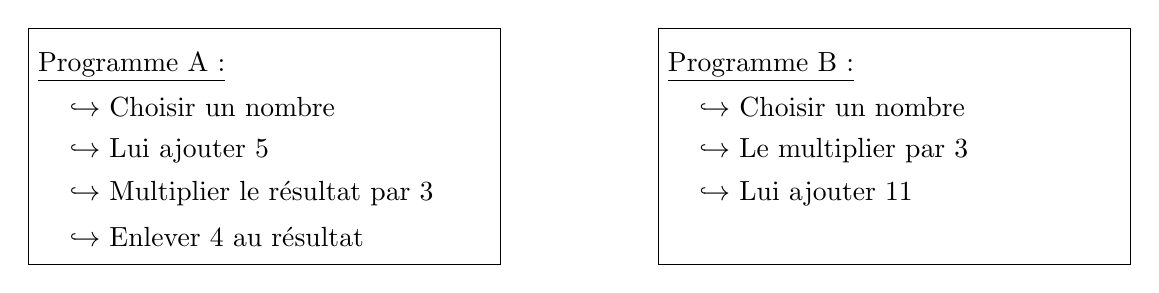
\begin{tikzpicture}
        \draw (0,0) rectangle +(6,3);
        \draw (8,0) rectangle +(6,3);
        \node[anchor=west] at (0,2.5) {\underline{Programme A :}};
        \node[anchor=west] at (8,2.5) {\underline{Programme B :}};
        \node[anchor=west] at (0.4,2) {$\hookrightarrow$ Choisir un nombre};
        \node[anchor=west] at (0.4,1.45) {$\hookrightarrow$ Lui ajouter 5};
        \node[anchor=west] at (0.4,0.9) {$\hookrightarrow$ Multiplier le résultat par 3};
        \node[anchor=west] at (0.4,0.35) {$\hookrightarrow$ Enlever 4 au résultat};
        \node[anchor=west] at (8.4,2) {$\hookrightarrow$ Choisir un nombre};
        \node[anchor=west] at (8.4,1.45) {$\hookrightarrow$ Le multiplier par 3};
        \node[anchor=west] at (8.4,0.9) {$\hookrightarrow$ Lui ajouter 11};
    \end{tikzpicture}
\end{center}

\question Appliquer les deux programmes de calcul au nombre 5.
\question Appliquer les deux programmes de calcul au nombre -2.
\question Appliquer les deux programmes de calcul au nombre $x$.
\question En utilisant le calcul littéral, montrer que les deux programmes donnent toujours le même résultat.

\exercicetitre{Partage équitable}

Un pirate et son équipage ont découvert un trésor composé de 135 pièces d'or et 459 pièces d'argent. 
\question Décomposer 135 et 459 en produit de facteurs premiers.
\question Quel est le plus grand diviseur en commun entre 135 et 459 ?
\question En supposant qu'il y a un nombre total de personnes égal à la réponse précédente, combien chacun aura-t-il de pièces d'or et d'argent ?

    \exercicetitre{Remplir une baignoire}
    Une baignoire dispose de 2 robinets : un pour l'eau chaude et un pour l'eau froide. 
    
    \question Le robinet d'eau chaude remplit la baignoire en 20 minutes, et le robinet d'eau froide remplit la baignoire en 15 minutes. \textbf{Combien de temps faut-il pour remplir la baignoire avec les deux robinets ?}

    \question Pour une baignoire de \qty{140}{\litre} remplie avec les deux robinets, \textbf{quelle quantité d'eau chaude et d'eau froide y aura-t-il ?}

    \question En supposant que l'eau chaude est à \qty{55}{\degreeCelsius} et l'eau froide à \qty{15}{\degreeCelsius}, quelle est la température de l'eau dans la baignoire une fois remplie ?


    \exercicetitre{Crédit}

    On souhaite acheter une maison d'une valeur de \qty{200000}{\EURO} net vendeur.

    \question L'agent immobilier prend une commission de \qty{5}{\percent} du net vendeur, c'est la valeur FAI (Frais d'Agence Inclus). Calculer cette valeur.

    \question Le notaire prend une commission de \qty{8}{\percent} du prix net vendeur, en ajoutant cela au frais d'agence, on obtient le prix que l'acheteur devra dépenser. Calculer cette valeur.

    \question Si une personne A rembourse le crédit seule en 25 ans, et qu'une personne B rembourse le crédit seule en 40 ans, combien de temps faudrait-il pour rembourser le crédit s'ils remboursent ensemble ?

\end{questions}
\end{document}

\end{document}